% Generated by LitigCharts.PublicationFigures. Captions and provenance are sidecars.
\documentclass[10pt,tikz,border=5pt]{standalone}
\usepackage{lmodern}
\usetikzlibrary{patterns,patterns.meta}
\begin{document}
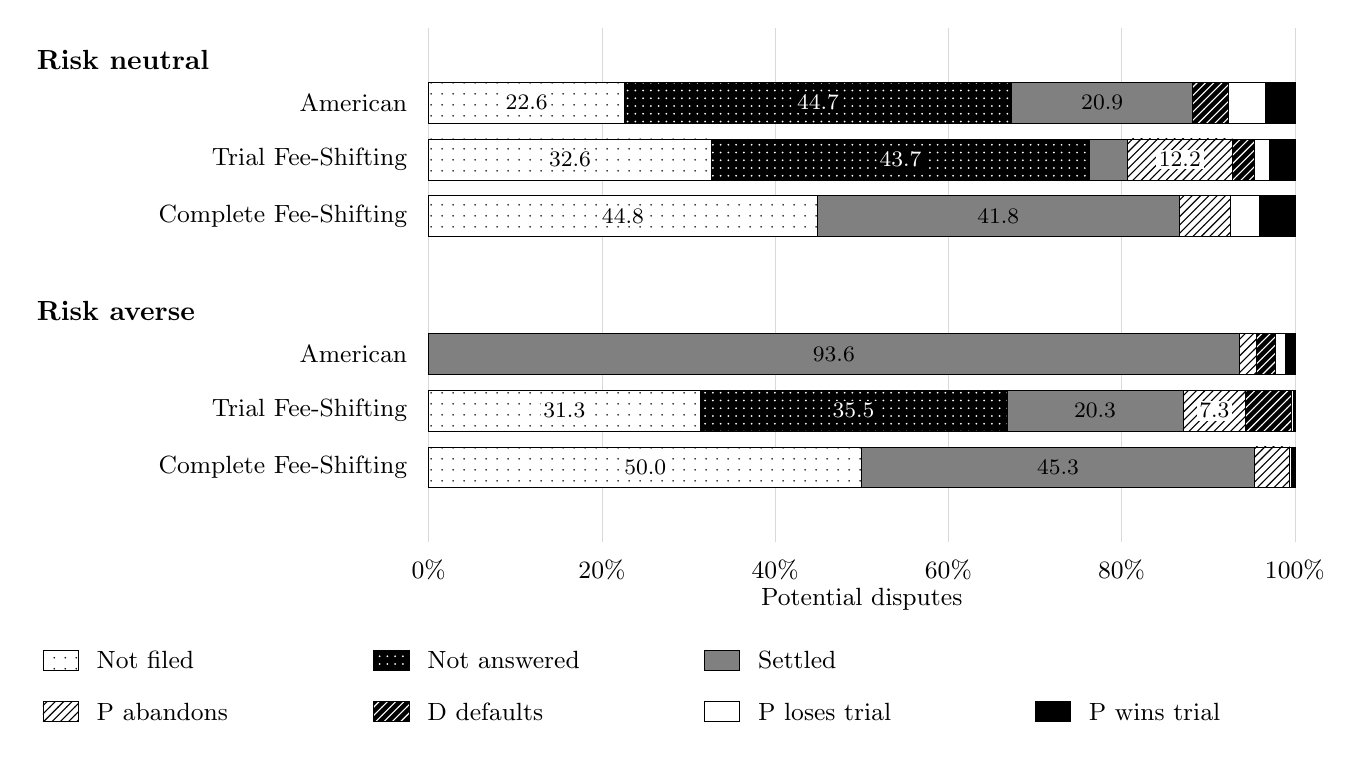
\begin{tikzpicture}[font=\small]\draw[black!15,line width=.2pt] (5.1,.65) -- (5.1,7.18);
\node[anchor=north] at (5.1,.55) {0\%};
\draw[black!15,line width=.2pt] (7.3,.65) -- (7.3,7.18);
\node[anchor=north] at (7.3,.55) {20\%};
\draw[black!15,line width=.2pt] (9.5,.65) -- (9.5,7.18);
\node[anchor=north] at (9.5,.55) {40\%};
\draw[black!15,line width=.2pt] (11.7,.65) -- (11.7,7.18);
\node[anchor=north] at (11.7,.55) {60\%};
\draw[black!15,line width=.2pt] (13.9,.65) -- (13.9,7.18);
\node[anchor=north] at (13.9,.55) {80\%};
\draw[black!15,line width=.2pt] (16.1,.65) -- (16.1,7.18);
\node[anchor=north] at (16.1,.55) {100\%};
\node[anchor=west,font=\bfseries] at (0,6.78) {\mbox{Risk} \mbox{neutral}};
\node[anchor=east] at (4.95,6.23) {American};
\path[preaction={fill=white,draw=none},pattern={Dots[distance=4pt,radius=.35pt]},pattern color=black,draw=black,line width=.25pt] (5.1,5.97) rectangle (7.58798,6.49);
\node[text=black,fill=white,font=\footnotesize,inner sep=1pt] at (6.34399,6.23) {22.6};
\path[preaction={fill=black,draw=none},pattern={Dots[distance=2.8pt,radius=.35pt]},pattern color=white,draw=black,line width=.25pt] (7.58798,5.97) rectangle (12.502868,6.49);
\node[text=white,fill=black,font=\footnotesize,inner sep=1pt] at (10.045424,6.23) {44.7};
\path[fill=black!50,draw=black,line width=.25pt] (12.502868,5.97) rectangle (14.802946,6.49);
\node[text=black,fill=none,font=\footnotesize,inner sep=1pt] at (13.652907,6.23) {20.9};
\path[preaction={fill=black,draw=none},pattern={north east lines},pattern color=white,draw=black,line width=.25pt] (14.802946,5.97) rectangle (15.25545,6.49);
\path[fill=white,draw=black,line width=.25pt] (15.25545,5.97) rectangle (15.724692,6.49);
\path[fill=black,draw=black,line width=.25pt] (15.724692,5.97) rectangle (16.100002,6.49);
\node[anchor=east] at (4.95,5.51) {Trial Fee-Shifting};
\path[preaction={fill=white,draw=none},pattern={Dots[distance=4pt,radius=.35pt]},pattern color=black,draw=black,line width=.25pt] (5.1,5.25) rectangle (8.69029,5.77);
\node[text=black,fill=white,font=\footnotesize,inner sep=1pt] at (6.895145,5.51) {32.6};
\path[preaction={fill=black,draw=none},pattern={Dots[distance=2.8pt,radius=.35pt]},pattern color=white,draw=black,line width=.25pt] (8.69029,5.25) rectangle (13.494837,5.77);
\node[text=white,fill=black,font=\footnotesize,inner sep=1pt] at (11.092564,5.51) {43.7};
\path[fill=black!50,draw=black,line width=.25pt] (13.494837,5.25) rectangle (13.970709,5.77);
\path[preaction={fill=white,draw=none},pattern={north east lines},pattern color=black,draw=black,line width=.25pt] (13.970709,5.25) rectangle (15.309423,5.77);
\node[text=black,fill=white,font=\footnotesize,inner sep=1pt] at (14.640066,5.51) {12.2};
\path[preaction={fill=black,draw=none},pattern={north east lines},pattern color=white,draw=black,line width=.25pt] (15.309423,5.25) rectangle (15.589052,5.77);
\path[fill=white,draw=black,line width=.25pt] (15.589052,5.25) rectangle (15.78141,5.77);
\path[fill=black,draw=black,line width=.25pt] (15.78141,5.25) rectangle (16.099992,5.77);
\node[anchor=east] at (4.95,4.79) {Complete Fee-Shifting};
\path[preaction={fill=white,draw=none},pattern={Dots[distance=4pt,radius=.35pt]},pattern color=black,draw=black,line width=.25pt] (5.1,4.53) rectangle (10.032873,5.05);
\node[text=black,fill=white,font=\footnotesize,inner sep=1pt] at (7.566437,4.79) {44.8};
\path[fill=black!50,draw=black,line width=.25pt] (10.032873,4.53) rectangle (14.636131,5.05);
\node[text=black,fill=none,font=\footnotesize,inner sep=1pt] at (12.334502,4.79) {41.8};
\path[preaction={fill=white,draw=none},pattern={north east lines},pattern color=black,draw=black,line width=.25pt] (14.636131,4.53) rectangle (15.28381,5.05);
\path[fill=white,draw=black,line width=.25pt] (15.28381,4.53) rectangle (15.653041,5.05);
\path[fill=black,draw=black,line width=.25pt] (15.653041,4.53) rectangle (16.100004,5.05);
\node[anchor=west,font=\bfseries] at (0,3.59) {\mbox{Risk} \mbox{averse}};
\node[anchor=east] at (4.95,3.04) {American};
\path[fill=black!50,draw=black,line width=.25pt] (5.1,2.78) rectangle (15.391303,3.3);
\node[text=black,fill=none,font=\footnotesize,inner sep=1pt] at (10.245652,3.04) {93.6};
\path[preaction={fill=white,draw=none},pattern={north east lines},pattern color=black,draw=black,line width=.25pt] (15.391303,2.78) rectangle (15.609989,3.3);
\path[preaction={fill=black,draw=none},pattern={north east lines},pattern color=white,draw=black,line width=.25pt] (15.609989,2.78) rectangle (15.850264,3.3);
\path[fill=white,draw=black,line width=.25pt] (15.850264,2.78) rectangle (15.978732,3.3);
\path[fill=black,draw=black,line width=.25pt] (15.978732,2.78) rectangle (16.099999,3.3);
\node[anchor=east] at (4.95,2.32) {Trial Fee-Shifting};
\path[preaction={fill=white,draw=none},pattern={Dots[distance=4pt,radius=.35pt]},pattern color=black,draw=black,line width=.25pt] (5.1,2.06) rectangle (8.545662,2.58);
\node[text=black,fill=white,font=\footnotesize,inner sep=1pt] at (6.822831,2.32) {31.3};
\path[preaction={fill=black,draw=none},pattern={Dots[distance=2.8pt,radius=.35pt]},pattern color=white,draw=black,line width=.25pt] (8.545662,2.06) rectangle (12.446207,2.58);
\node[text=white,fill=black,font=\footnotesize,inner sep=1pt] at (10.495935,2.32) {35.5};
\path[fill=black!50,draw=black,line width=.25pt] (12.446207,2.06) rectangle (14.678371,2.58);
\node[text=black,fill=none,font=\footnotesize,inner sep=1pt] at (13.562289,2.32) {20.3};
\path[preaction={fill=white,draw=none},pattern={north east lines},pattern color=black,draw=black,line width=.25pt] (14.678371,2.06) rectangle (15.475948,2.58);
\node[text=black,fill=white,font=\footnotesize,inner sep=1pt] at (15.07716,2.32) {7.3};
\path[preaction={fill=black,draw=none},pattern={north east lines},pattern color=white,draw=black,line width=.25pt] (15.475948,2.06) rectangle (16.051239,2.58);
\path[fill=white,draw=black,line width=.25pt] (16.051239,2.06) rectangle (16.075661,2.58);
\path[fill=black,draw=black,line width=.25pt] (16.075661,2.06) rectangle (16.09999,2.58);
\node[anchor=east] at (4.95,1.6) {Complete Fee-Shifting};
\path[preaction={fill=white,draw=none},pattern={Dots[distance=4pt,radius=.35pt]},pattern color=black,draw=black,line width=.25pt] (5.1,1.34) rectangle (10.6,1.86);
\node[text=black,fill=white,font=\footnotesize,inner sep=1pt] at (7.85,1.6) {50.0};
\path[fill=black!50,draw=black,line width=.25pt] (10.6,1.34) rectangle (15.58212,1.86);
\node[text=black,fill=none,font=\footnotesize,inner sep=1pt] at (13.09106,1.6) {45.3};
\path[preaction={fill=white,draw=none},pattern={north east lines},pattern color=black,draw=black,line width=.25pt] (15.58212,1.34) rectangle (16.033644,1.86);
\path[fill=white,draw=black,line width=.25pt] (16.033644,1.34) rectangle (16.053052,1.86);
\path[fill=black,draw=black,line width=.25pt] (16.053052,1.34) rectangle (16.099995,1.86);
\node at (10.6,-.08) {Potential disputes};
\path[preaction={fill=white,draw=none},pattern={Dots[distance=4pt,radius=.35pt]},pattern color=black,draw=black,line width=.25pt] (0.2,-0.98) rectangle (0.65,-0.72);
\node[anchor=west] at (0.76,-0.85) {Not filed};
\path[preaction={fill=black,draw=none},pattern={Dots[distance=2.8pt,radius=.35pt]},pattern color=white,draw=black,line width=.25pt] (4.4,-0.98) rectangle (4.85,-0.72);
\node[anchor=west] at (4.96,-0.85) {Not answered};
\path[fill=black!50,draw=black,line width=.25pt] (8.6,-0.98) rectangle (9.05,-0.72);
\node[anchor=west] at (9.16,-0.85) {Settled};
\path[preaction={fill=white,draw=none},pattern={north east lines},pattern color=black,draw=black,line width=.25pt] (0.2,-1.63) rectangle (0.65,-1.37);
\node[anchor=west] at (0.76,-1.5) {P abandons};
\path[preaction={fill=black,draw=none},pattern={north east lines},pattern color=white,draw=black,line width=.25pt] (4.4,-1.63) rectangle (4.85,-1.37);
\node[anchor=west] at (4.96,-1.5) {D defaults};
\path[fill=white,draw=black,line width=.25pt] (8.6,-1.63) rectangle (9.05,-1.37);
\node[anchor=west] at (9.16,-1.5) {P loses trial};
\path[fill=black,draw=black,line width=.25pt] (12.8,-1.63) rectangle (13.25,-1.37);
\node[anchor=west] at (13.36,-1.5) {P wins trial};
\end{tikzpicture}
\end{document}
